\begin{pastexam}[label={px:gw3-103-ds-03}]{關務三等資訊處理 103 年 第三題}
（申論；20 分）

\begin{itemize}[leftmargin=2.2em]
\item[㈠] 請繪出一二元樹來表示運算式（expression）$-$a+b/(c$-$d)$-$a*b/c+d。（8 分）
\item[㈡] 請列出此二元樹的後序走訪（postorder traversal）、深度優先走訪（depth-first search traversal）及廣度優先走訪
（breadth-first search traversal）。（12 分）
\end{itemize}
\end{pastexam}

\begin{pastsoln}
答案：㈠ 樹如下圖（最前面的 $-$ 是一元負號，記為 $\ominus$，只有一個子節點）。 ㈡ 後序
a $\ominus$ b c d $-$ / + a b * c / $-$ d +；深度優先（前序）+ $-$ + $\ominus$ a / b $-$ c d / * a b c d；廣度優先
+ $-$ d + / $\ominus$ / * c a b $-$ a b c d。

\textbf{㈠ 加括號。} 依一般的優先順序：一元負號最高，再來 $*$、$/$，最後 $+$、$-$；同級由左而右結合（資結書第~6.3、
7.7~節）。 開頭的 $-$ 前面沒有運算元，是\textbf{一元負號}，只作用在 a 上。 完整加括號：
\[
\Bigl(\bigl((-a) + (b / (c - d))\bigr) - \bigl((a * b) / c\bigr)\Bigr) + d .
\]
最後做的運算是最外層的 $+$，它是根；左子樹是 $\bigl((-a) + b/(c-d)\bigr) - (a*b)/c$，右子樹是 d。 依此一層一層拆：
\begin{center}
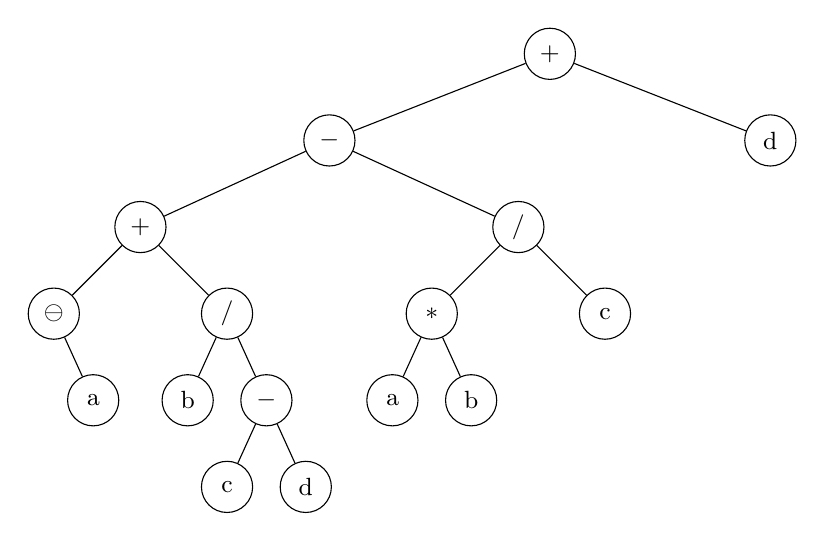
\begin{tikzpicture}[v/.style={circle,draw,minimum size=6.5mm,inner sep=0pt,font=\small},
  level distance=11mm, level 1/.style={sibling distance=56mm}, level 2/.style={sibling distance=48mm},
  level 3/.style={sibling distance=22mm}, level 4/.style={sibling distance=10mm}, level 5/.style={sibling distance=10mm}]
\node[v] {$+$}
  child {node[v] {$-$}
    child {node[v] {$+$}
      child {node[v] {$\ominus$} child[missing] {} child {node[v] {a}}}
      child {node[v] {/} child {node[v] {b}} child {node[v] {$-$} child {node[v] {c}} child {node[v] {d}}}}}
    child {node[v] {/}
      child {node[v] {$*$} child {node[v] {a}} child {node[v] {b}}}
      child {node[v] {c}}}}
  child {node[v] {d}};
\end{tikzpicture}
\end{center}
一元負號 $\ominus$ 只有一個運算元，畫成只有一個子節點；放在右邊，中序走訪時才會讀成「$-$a」。 檢查：中序走訪（左、根、
右）得 $\ominus$ a + b / c $-$ d $-$ a * b / c + d，補上括號就是原式。 （也有書把 $-a$ 寫成 $0 - a$，用一般的二元
$-$ 節點、左子節點放 $0$；答題時寫明採用哪一種即可。）

\textbf{㈡} 三種走訪（資結書第~7.3~節）：
\begin{itemize}
\item \textbf{後序}（左、右、根）：
\[
\text{a}\ \ominus\ \text{b}\ \text{c}\ \text{d}\ -\ /\ +\ \text{a}\ \text{b}\ *\ \text{c}\ /\ -\ \text{d}\ +
\]
這就是原式的後序（逆波蘭）表示法。
\item \textbf{深度優先}：從根開始，先走完左子樹再走右子樹，每個節點第一次碰到時就拜訪，也就是\textbf{前序}（根、左、右）：
\[
+\ -\ +\ \ominus\ \text{a}\ /\ \text{b}\ -\ \text{c}\ \text{d}\ /\ *\ \text{a}\ \text{b}\ \text{c}\ \text{d}
\]
\item \textbf{廣度優先}：一層一層、每層由左而右（資結書第~7.3.2~節）：
\begin{center}
\small
\begin{tabular}{cl}
\toprule
層 & 節點 \\
\midrule
1 & $+$ \\
2 & $-$,\ d \\
3 & $+$,\ / \\
4 & $\ominus$,\ /,\ $*$,\ c \\
5 & a,\ b,\ $-$,\ a,\ b \\
6 & c,\ d \\
\bottomrule
\end{tabular}
\end{center}
所以是
\[
+\ -\ \text{d}\ +\ /\ \ominus\ /\ *\ \text{c}\ \text{a}\ \text{b}\ -\ \text{a}\ \text{b}\ \text{c}\ \text{d}
\]
\end{itemize}
（深度優先走訪若約定「先拜訪子節點再拜訪自己」，得到的就是後序；一般說樹的深度優先走訪指的是前序。）
\end{pastsoln}
